\documentclass[a4paper,11pt, spanish]{article}
\usepackage[spanish]{babel}
\usepackage{graphicx}
\selectlanguage{spanish}
\usepackage[utf8]{inputenc}
% Title Page
\title{Central Meteorológica con fines educativos}
\author{Raul Giucich}


\begin{document}

\section{Integrantes}
Raúl Ricardo Giucich González
CO2383 - CI.:1147658

\section{Título del trabajo}
Central Meteorológica con fines educativos

\section{Tutor}
Profesor Licenciado Hugo Javier Díaz Lavigne

\section{Fecha}
14 de Abril de 2014

\section{Justificación del trabajo}
El objetivo de esta Tesis es construir una central meteorológica con elementos que en su gran mayoría se pueden conseguir en ferreterías y negocios de electrónica locales. Los sensores, MODEM y el PIC que los controla son los únicos elementos importados. Todo el software y hardware producido y utilizado durante este trabajo será Open Source y Open Hardware respectivamente, convirtiéndose en un nodo más de "Internet of Things"

La audiencia de este producto es la educación escolar básica (EEB), tanto docentes como alumos a partir de los 12 años, y será un medio para introdudir en la escuela la electrónica y la informática desde un enfoque de producción y no de consumo. El uso de estos productos complementarán las materias de matemática, medio natural, ciencias de la salud y estimularán el uso del método científico. La construcción estimulará el trabajo en equipo y habilidades relacionadas al trabajo técnico como la presición, la medición y el diagnóstico.

La Central tendrá conexión a Internet y podrá enviar los datos a una aplicación web de soporte que contendrá la geolocalización de las centrales, materiales educativos relacionados al clima, visualización y acceso a datos.

\section{Descripción del trabajo}
El trabajo se compone de 3 elementos:
\begin{enumerate}
\item Central propiamente dicha:
\begin{itemize}
\item Mediciones: Velocidad del viento, dirección del viento, temperatura, humedad relativa ambiente, cantidad de lluvia y calidad del aire (NO2 - Dióxido de Nitrógeno y CO2 - Anhidrido carbónico).
\item Control: Arduino UNO utilizando los puertos analógicos y digitales para la captura.
\item Conexiones: Conectores RJ11 de 4 hilos (V+, GND, DATA, AUX).
\item Montaje: Componentes soldados sobre tarjetas perforadas.
\item Fuente: Fuente de corriente 9v, 650mA.
\item Transmisión de datos: Ethernet Shield de Arduino o Puerto Ethernet de NANODE, Modem GSM.
\item Infraestructura: Pagoda para los sensores de temperatura, humedad y calidad del aire. El pluviómetro, velocidad y dirección del viento utilizando latas con estructura interna reforzada, caños de PVC para la elevación.
\item Software: utilizando Arduino Programming Language y SDK Arduino.
\item Normalización de datos: Utilizar open data con nivel de 4 estrellas de las 5 de 5stardata.info
\end{itemize}
\item Manual de construcción de la Central y conectividad a Internet.
\begin{itemize}
\item Lista de compra de materiales y herramientas a utilizar.
\item Esquemáticos de los circuitos.
\item Guía de soldado, verificación y montaje de componentes.
\item Guía de construcción y montaje de la infraestructura.
\item Registro de la central en la APP web y uso de la API para la publicación y consumo de los datos.
\end{itemize}
\item Aplicación WEB de soporte para almacenamiento de datos y publicación de los mismos.
\begin{itemize}
\item Registro de una central: Geolocalización y disponibilidad de sensores.
\item Agregación de datos capturados para cumplimiento de estrellas de Open Data
\item Visualización de datos capturados
\item Descarga en archivos y API de acceso a datos.
\item Material educativo de referencia para la utilización de los datos en el aula.
\item Software: Framework Laravel 4, Postgres, Postgis, AngularJS, ZURB Foundation. Publicado en yvytu.net
\end{itemize}
\end{enumerate}

\section{Alcance}
Inicia con la Investigación sobre como funciona una central meteorológica, la disponibilidad de sensores, la captura de datos meteorológicos, el aprendizaje experiencial en el aula (el uso de datos ambientales y la enseñanza de electrónica e informática) y la normalización de datos para Open Data.
Como productos entregables
\begin{enumerate}
\item Una central montada y en funcionamiento en el predio de un colegio en la ciudad de Lambaré o en la Universidad.
\item Aplicación WEB publicada en Internet.
\item Copia del manual publicada.
\end{enumerate}

\section{Esquema Gráfico}
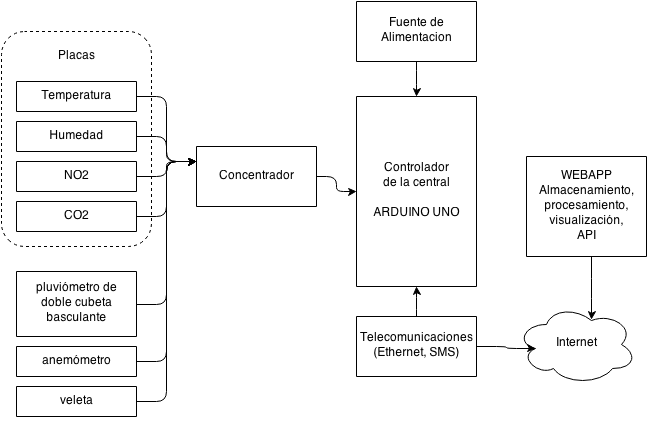
\includegraphics[width=0.9\textwidth,natwidth=648,natheight=421]{Central.png}

\section{Recursos Metodológicos}
Se realizará una investigación de carácter documental sobre los elementos descriptos en el alcance, para el desarrollo del software de la central se utilizará una arquitectura basada en interrupciones debido a la cantidad de sensores que proveen datos de entrada concurrentemente.

Para la Aplicación WEB se utilizará Orientación a Objetos y para la organización del Proyecto se utilizará SCRUM, proponiendo que el Tutor sea el SCRUM Master con quién discutir las dificultades y acordar las funcionalidades a implementar en cada Sprint.  

\section{Cronograma de tareas}
\begin{enumerate}
\item \textbf{Inicio}: 28/04, \textbf{Duración}: 5D, \textbf{Actividad}: Investigación sobre la Historia, características y componentes de una central meteorológica y sensores sobre la calidad del aire, \textbf{Recursos}: Internet, Biblioteca UCA, \textbf{PreRequisitos}: Ninguno
\item \textbf{Inicio}: 05/05, \textbf{Duración}: 1D, \textbf{Actividad}: Relevamiento de sensores, hojas técnicas de los mismos, costos y diagramas de montaje de los componentes de la central, \textbf{Recursos}: Internet, Biblioteca UCA, \textbf{PreRequisitos}: Tarea 1.
\item \textbf{Inicio}: 06/05, \textbf{Duración}: 13D, \textbf{Actividad}: Diseño de placas de sensores incluyendo la lista de materiales, esquemáticos, diagramas de soldadura para tarjeta perforada y método de testeo, \textbf{Recursos}: KICAD, InkScape, \textbf{PreRequisitos}: Tarea 2
\item \textbf{Inicio}: 19/05, \textbf{Duración}: 4D, \textbf{Actividad}: Montaje de las placas para los sensores, \textbf{Recursos}: diagramas de soldadura, componentes, soldador, estaño, multímetro digital, \textbf{PreRequisitos}: Tarea 3
\item Inicio: 24/05, Duración: 7D, Actividad:  
\end{enumerate}
\end{document}          
